% THIS DOCUMENT IS TAILORED TO REQUIREMENTS FOR SCIENTIFIC COMPUTING.  IT SHOULDN'T
% BE USED FOR NON-SCIENTIFIC COMPUTING PROJECTS
\documentclass[12pt]{article}

\usepackage{amsmath, mathtools}
\usepackage{amsfonts}
\usepackage{amssymb}
\usepackage{graphicx}
\usepackage{colortbl}
\usepackage{xr}
\usepackage{hyperref}
\usepackage{longtable}
\usepackage{xfrac}
\usepackage{tabularx}
\usepackage{float}
\usepackage{siunitx}
\usepackage{booktabs}
\usepackage{caption}
\usepackage{pdflscape}
\usepackage{afterpage}

\usepackage[round]{natbib}

%\usepackage{refcheck}

\hypersetup{
    bookmarks=true,         % show bookmarks bar?
      colorlinks=true,       % false: boxed links; true: colored links
    linkcolor=red,          % color of internal links (change box color with linkbordercolor)
    citecolor=green,        % color of links to bibliography
    filecolor=magenta,      % color of file links
    urlcolor=cyan           % color of external links
}

\input{../Comments}
%% Common Parts

\newcommand{\progname}{Baja Dynamics} % PUT YOUR PROGRAM NAME HERE
\newcommand{\authname}{Team \#17, Team Name
\\ Grace McKenna
\\ Travis Wing
\\ Cameron Dunn
\\ Kai Arseneau} % AUTHOR NAMES                  

\usepackage{hyperref}
    \hypersetup{colorlinks=true, linkcolor=blue, citecolor=blue, filecolor=blue,
                urlcolor=blue, unicode=false}
    \urlstyle{same}
                                


% For easy change of table widths
\newcommand{\colZwidth}{1.0\textwidth}
\newcommand{\colAwidth}{0.13\textwidth}
\newcommand{\colBwidth}{0.82\textwidth}
\newcommand{\colCwidth}{0.1\textwidth}
\newcommand{\colDwidth}{0.05\textwidth}
\newcommand{\colEwidth}{0.8\textwidth}
\newcommand{\colFwidth}{0.17\textwidth}
\newcommand{\colGwidth}{0.5\textwidth}
\newcommand{\colHwidth}{0.28\textwidth}

% Used so that cross-references have a meaningful prefix
\newcounter{defnum} %Definition Number
\newcommand{\dthedefnum}{GD\thedefnum}
\newcommand{\dref}[1]{GD\ref{#1}}
\newcounter{datadefnum} %Datadefinition Number
\newcommand{\ddthedatadefnum}{DD\thedatadefnum}
\newcommand{\ddref}[1]{DD\ref{#1}}
\newcounter{theorynum} %Theory Number
\newcommand{\tthetheorynum}{TM\thetheorynum}
\newcommand{\tref}[1]{TM\ref{#1}}
\newcounter{tablenum} %Table Number
\newcommand{\tbthetablenum}{TB\thetablenum}
\newcommand{\tbref}[1]{TB\ref{#1}}
\newcounter{assumpnum} %Assumption Number
\newcommand{\atheassumpnum}{A\theassumpnum}
\newcommand{\aref}[1]{A\ref{#1}}
\newcounter{goalnum} %Goal Number
\newcommand{\gthegoalnum}{GS\thegoalnum}
\newcommand{\gsref}[1]{GS\ref{#1}}
\newcounter{instnum} %Instance Number
\newcommand{\itheinstnum}{IM\theinstnum}
\newcommand{\iref}[1]{IM\ref{#1}}
\newcounter{reqnum} %Requirement Number
\newcommand{\rthereqnum}{R\thereqnum}
\newcommand{\rref}[1]{R\ref{#1}}
\newcounter{nfrnum} %NFR Number
\newcommand{\rthenfrnum}{NFR\thenfrnum}
\newcommand{\nfrref}[1]{NFR\ref{#1}}
\newcounter{lcnum} %Likely change number
\newcommand{\lthelcnum}{LC\thelcnum}
\newcommand{\lcref}[1]{LC\ref{#1}}

\usepackage{fullpage}

\newcommand{\deftheory}[9][Not Applicable]
{
\newpage
\noindent \rule{\textwidth}{0.5mm}

\paragraph{RefName: } \textbf{#2} \phantomsection 
\refstepcounter{theorynum} \label{#2}

\paragraph{Label:} #3

\noindent \rule{\textwidth}{0.5mm}

\paragraph{Equation:}

#4

\paragraph{Description:}

#5

\paragraph{Notes:}

#6

\paragraph{Source:}

#7

\paragraph{Ref.\ By:}

#8

\paragraph{Preconditions for \hyperref[#2]{#2}:}
\label{#2_precond}

#9

\paragraph{Derivation for \hyperref[#2]{#2}:}
\label{#2_deriv}

#1

\noindent \rule{\textwidth}{0.5mm}

}

\newcommand{\definstance}[7] {
~\newline
\noindent
\begin{minipage}{\textwidth}
\renewcommand*{\arraystretch}{1.5}
\begin{tabular}{| p{\colAwidth} | p{\colBwidth}|}
  \hline
  \rowcolor[gray]{0.9}
  Number& IM\refstepcounter{instnum}\theinstnum \label{inst:\theinstnum}\\
  \hline
  Label& \bf #1 \\
  \hline
  Input& #2\\
  \hline
  Equation& #3\\
  \hline
  Output& #4\\
  \hline
  Description& #5 \\
  \hline
  Sources& #6 \\
  \hline
  Ref.\ By & #7\\
  \hline
\end{tabular}
\end{minipage}\\

}

\begin{document}

\title{Software Requirements Specification for \progname: subtitle describing software} 
\author{\authname}
\date{\today}
	
\maketitle

~\newpage

\pagenumbering{roman}

\tableofcontents

~\newpage

\section*{Revision History}

\begin{tabularx}{\textwidth}{p{3cm}p{2cm}X}
\toprule {\bf Date} & {\bf Version} & {\bf Notes}\\
\midrule
Date 1 & 1.0 & Notes\\
Date 2 & 1.1 & Notes\\
\bottomrule
\end{tabularx}

~\\

~\newpage

\section{Reference Material}

This section records information for easy reference.

\subsection{Table of Units}

Throughout this document SI (Syst\`{e}me International d'Unit\'{e}s) is employed
as the unit system.  In addition to the basic units, several derived units are
used as described below.  For each unit, the symbol is given followed by a
description of the unit and the SI name.
~\newline

\renewcommand{\arraystretch}{1.2}
%\begin{table}[ht]
  \noindent \begin{tabular}{l l l} 
    \toprule		
    \textbf{symbol} & \textbf{unit} & \textbf{SI}\\
    \midrule 
    \si{\metre} & length & metre\\
    \si{\kilogram} & mass	& kilogram\\
    \si{\second} & time & second\\
    \si{\celsius} & temperature & centigrade\\
    \si{\joule} & energy & joule\\
    \si{\watt} & power & watt (W = \si{\joule\per\second})\\
    \si{\newton} & force & newtons (N = \si{\kilogram \metre\per\square\second} )\\
    Nm & torque & newton metre (Nm = \si{\kilogram \square\metre\per\square\second})\\
    \si{\radian} & angle & radian\\
    \bottomrule
  \end{tabular}
  %	\caption{Provide a caption}
%\end{table}

\plt{Only include the units that your SRS actually uses.}

\plt{Derived units, like newtons, pascal, etc, should show their derivation
    (the units they are derived from) if their constituent units are in the
    table of units (that is, if the units theye derived from are used in the
    document).  For instance, the derivation of pascals as
    $\si{\pascal}=\si{\newton\per\square\meter}$ is shown if newtons and m are
    both in the table.  The derivations of newtons would not be shown if kg and
    s are not both in the table.}

\plt{The symbol for units named after people use capital letters, but the name
  of the unit itself uses lower case.  For instance, pascals use the symbol Pa,
  watts use the symbol W, teslas use the symbol T, newtons use the symbol N,
  etc.  The one exception to this is degree Celsius.  Details on writing metric
  units can be found on the 
  \href{https://www.nist.gov/pml/weights-and-measures/writing-metric-units}
  {NIST} web-page.}

\subsection{Table of Symbols}

The table that follows summarizes the symbols used in this document along with
their units.  The choice of symbols was made to be consistent with the heat
transfer literature and with existing documentation for solar water heating
systems.  The symbols are listed in alphabetical order.

\renewcommand{\arraystretch}{1.2}
%\noindent \begin{tabularx}{1.0\textwidth}{l l X}
\noindent \begin{longtable*}{l l p{12cm}} \toprule
\textbf{symbol} & \textbf{unit} & \textbf{description}\\
\midrule 
$A_C$ & \si[per-mode=symbol] {\square\metre} & coil surface area
\\
$A_\text{in}$ & \si[per-mode=symbol] {\square\metre} & surface area over 
which heat is transferred in
\\ 
\bottomrule
\end{longtable*}
\plt{Use your problems actual symbols.  The si package is a good idea to use for
  units.}

\subsection{Abbreviations and Acronyms}

\renewcommand{\arraystretch}{1.2}
\begin{tabular}{l l} 
  \toprule		
  \textbf{symbol} & \textbf{description}\\
  \midrule 
  A & Assumption\\
  DD & Data Definition\\
  GD & General Definition\\
  GS & Goal Statement\\
  IM & Instance Model\\
  LC & Likely Change\\
  PS & Physical System Description\\
  R & Requirement\\
  SRS & Software Requirements Specification\\
  TM & Theoretical Model\\
  RPM & Revolutions Per Minute\\
  CVT & Continuous Variable Transmission\\
  SEC & Secondary\\
  PRIM & Primary\\
  \bottomrule
\end{tabular}\\

\subsection{Mathematical Notation}

N/A

\newpage

\pagenumbering{arabic}

\plt{This SRS template is based on \citet{SmithAndLai2005, SmithEtAl2007,
  SmithAndKoothoor2016}.  It will get you started.  You should not modify the
  section headings, without first discussing the change with the course
  instructor.  Modification means you are not following the template, which
  loses some of the advantage of a template, especially standardization.
  Although the bits shown below do not include type information, you may need to
  add this information for your problem.  If you are unsure, please can ask the
  instructor.}

\plt{Feel free to change the appearance of the report by modifying the LaTeX
  commands.}

\plt{This template document assumes that a single program is being documented.
  If you are documenting a family of models, you should start with a commonality
  analysis.  A separate template is provided for this.  For program
  families you should look at \cite{Smith2006, SmithMcCutchanAndCarette2017}.
  Single family member programs are often programs based on a single physical
  model.  General purpose tools are usually documented as a family.  Families of
  physical models also come up.}

\plt{The SRS is not generally written, or read, sequentially.  The SRS is a
  reference document.  It is generally read in an ad hoc order, as the need
  arises.  For writing an SRS, and for reading one for the first time, the
  suggested order of sections is:
\begin{itemize}
\item Goal Statement
\item Instance Models
\item Requirements
\item Introduction
\item Specific System Description
\end{itemize}
}

\plt{Guiding principles for the SRS document:
\begin{itemize}
\item Do not repeat the same information at the same abstraction level.  If
  information is repeated, the repetition should be at a different abstraction
  level.  For instance, there will be overlap between the scope section and the
  assumptions, but the scope section will not go into as much detail as the
  assumptions section.
\end{itemize}
}

\plt{The template description comments should be disabled before submitting this
  document for grading.}

\plt{You can borrow any wording from the text given in the template.  It is part
  of the template, and not considered an instance of academic integrity.  Of
  course, you need to cite the source of the template.}

\plt{When the documentation is done, it should be possible to trace back to the
  source of every piece of information.  Some information will come from
  external sources, like terminology.  Other information will be derived, like
  General Definitions.}

\plt{An SRS document should have the following qualities: unambiguous,
  consistent, complete, validatable, abstract and traceable.}

\plt{The overall goal of the SRS is that someone that meets the Characteristics
  of the Intended Reader (Section~\ref{sec_IntendedReader}) can learn,
  understand and verify the captured domain knowledge.  They should not have to
  trust the authors of the SRS on any statements.  They should be able to
  independently verify/derive every statement made.}

\section{Introduction}

The McMaster Baja engineering team is facing challenges in tuning their Continuous Variable Transmission (CVT). 
The current process of tuning the CVT is extensive, time consuming and requires testing of multiple physical components leading to possible inconsistencies due to weather and wear. 
These inconsistences then complicate the tuning process of the CVT’s torque transfer directly affecting the performance of the Baja vehicles. 
To address these issues, our team aims to develop a CVT simulation tool that uses mathematical models, a rendering engine and a user-friendly interface. 
Our solution aims to streamline the optimization process allowing Baja members to simulate real-world factors and virtually test various tuning parameters. 
Our simulation tool will be validated against data collected by the McMaster Baja Data Acquisition team to ensure reliability and accuracy.  
\\
\\
This introduction will outline the key objectives of this document to provide a structured guide for the development of the CVT tool and outline of the system’s requirements. 
Additionally, the scope will explore technical and functional assumptions and will intend to streamline the complex tuning process of a CVT. 
A detailed overview of this document will provide guidance to the reader regarding the structure and flow of the document. 

\subsection{Purpose of Document}

The purpose of this Software Requirements Specification (SRS) is to provide an outline of the system requirements given for the development of a CVT simulation tool. 
This ensures that all stakeholders including members of the Baja team, Dr.Smith and the developers understand the projects objectives and constraints. 
This document will serve as a communication tool to align expectations, provide guidance during the design of this tool and aid in the development and testing phases of this project. 
This SRS will be referenced throughout the development of the system to ensure the tool is within the scope and meets the outlined requirements. 

\subsection{Scope of Requirements}

\plt{Modelling the real world requires simplification.  The full complexity of
  the actual physics, chemistry, biology is too much for existing models, and
  for existing computational solution techniques.  Rather than say what is in
  the scope, it is usually easier to say what is not.  You can think of it as
  the scope is initially everything, and then it is constrained to create the
  actual scope.  For instance, the problem can be restricted to 2 dimensions, or
  it can ignore the effect of temperature (or pressure) on the material
  properties, etc.}  

\plt{The scope section is related to the assumptions section
  (Section~\ref{sec_assumpt}).  However, the scope and the assumptions are not
  at the same level of abstraction.  The scope is at a high level.  The focus is
  on the ``big picture'' assumptions.  The assumptions section lists, and
  describes, all of the assumptions.}

\plt{The scope section is relevant for later determining typical values of inputs. The scope should make it clear what inputs are reasonable to expect. This is a distinction between scope and context (context is a later section).  Scope affects the inputs while context affects how the software will be used.}

This model will simulate as a closed system and will not consider environmental factors such as temperature, humidity, and wind.
It also will not consider any unintended damage, forces or effects on the components of the CVT system.
The system will not account for any relative displacement between the components of the CVT system due to driver input or external forces.

\subsection{Characteristics of Intended Reader} \label{sec_IntendedReader}

Readers or reviewers of this SRS document should have a solid understanding of the principles of physics and calculus.
Knowledge of the components in a Continuous Variable Transmission (CVT) and a basic understanding of how these parts work together will also be beneficial. 
Proficiency in these areas will enough to comprehend the material in this document.

\subsection{Organization of Document}

This document is structured as follows:
\begin{itemize}
  \item Section 3 discusses the general context and description of the system
  \item Section 4 details the specific system description, goals, and definitions
  \item Section 5 covers the system requirements
  \item Section 6 outlines the likely changes for the system
  \item Section 7 discusses the unlikely changes for the system
  \item Section 8 covers the traceability of the requirements
\end{itemize}

\section{General System Description}

This section provides general information about the system.  It identifies the
interfaces between the system and its environment, describes the user
characteristics and lists the system constraints.

\subsection{System Context}

\begin{figure}[h!]
\begin{center}
 \includegraphics[width=0.9\textwidth]{{SystemContextFigure}}
\caption{System Context}
\label{Fig_SystemContext} 
\end{center}
\end{figure}

\begin{itemize}
\item User Responsibilities:
\begin{itemize}
\item Provide the necessary input data in a correct format.
\end{itemize}
\item \progname{} Responsibilities:
\begin{itemize}
\item Accept user input data to simulate the CVT system.
\item Display the results of the simulation.
\end{itemize}
\end{itemize}

\subsection{User Characteristics} \label{SecUserCharacteristics}

The expected user of this application is someone who is very familiar with drivetrains and CVTs but not necessarily familiar with software.
The software expects the user to know all of the components of a CVT and how they can be modified or adjusted.
The user should also have enough of an understanding of undergraduate physics and calculus to be able to make sense of the outputs of the software.
On the software side, the user should be able to navigate a GUI and know how to input data into the software.

\subsection{System Constraints}

The system should be able to run on any machine that supports Python 3.9 or later and Unity projects.

\section{Specific System Description}

This section first presents the problem description, which gives a high-level
view of the problem to be solved.  This is followed by the solution characteristics
specification, which presents the assumptions, theories, definitions and finally
the instance models. 

\subsection{Problem Description} \label{Sec_pd}

The CVT simulator is intended to address the challenges faced by the McMaster Baja racing team when they tune there CVT.
The current tuning process is time-consuming and requires physical testing of multiple components and configurations. This leads to inconsistencies in the tuning process due to weather and wear.
The CVT simulator will allow the Baja team to virtually test different tuning parameters and simulate real-world factors that affect the CVT's performance.

\subsubsection{Terminology and  Definitions}

\plt{This section is expressed in words, not with equations.  It provide the
  meaning of the different words and phrases used in the domain of the problem.
The terminology is used to introduce concepts from the world outside of the
mathematical model  The terminology provides a real world connection to give the
mathematical model meaning.}

This subsection provides a list of terms that are used in the subsequent
sections and their meaning, with the purpose of reducing ambiguity and making it
easier to correctly understand the requirements:

\begin{itemize}
  \item rpm
  \item CVT
  \item torque
  \item Primary RPM
  \item Secondary RPM
  \item Belt
  \item Ramp
  \item Fly Weight
\end{itemize}
  \begin{itemize}

\item 

\end{itemize}
\begin{figure}[h!]
  \begin{center}
      \begin{minipage}{0.45\textwidth}
          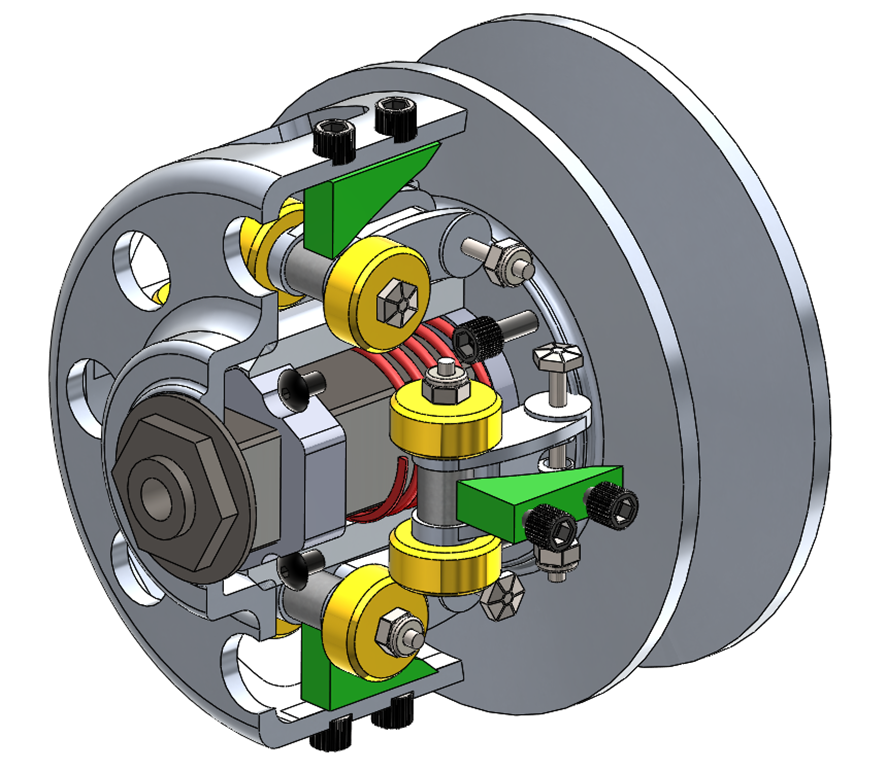
\includegraphics[scale=0.5]{primaryCVT.png}
          \caption{Primary CVT}
          \label{Fig_PrimaryCVT}
      \end{minipage}
      \hfill % This adds space between the figures
      \begin{minipage}{0.45\textwidth}
          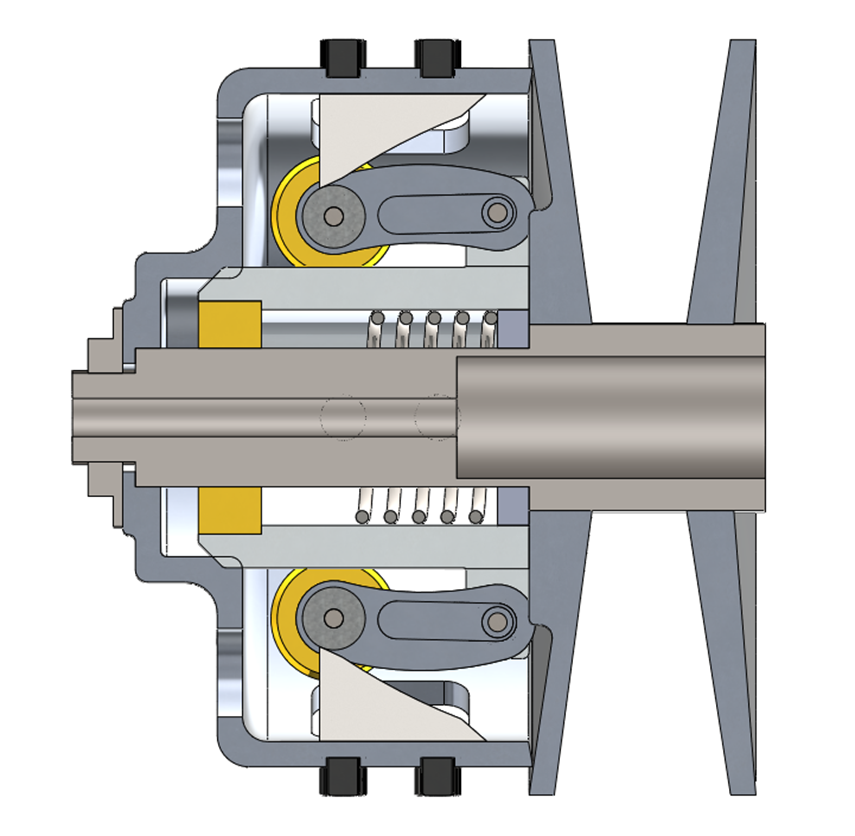
\includegraphics[scale=0.5]{primaryCVTSideView.png}
          \caption{Primary CVT Side View}
          \label{Fig_PrimaryCVTSideView}
      \end{minipage}
  \end{center}
\end{figure}

\begin{figure}[h!]
  \begin{center}
      \begin{minipage}{0.45\textwidth}
          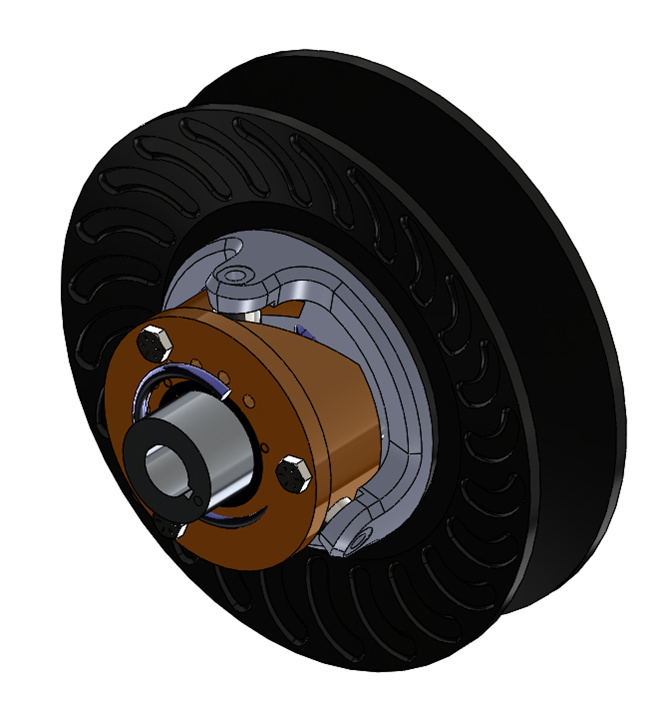
\includegraphics[scale=0.5]{secondaryCVT.png}
          \caption{Secondary CVT}
          \label{Fig_SecondaryCVT}
      \end{minipage}
      \hfill % This adds space between the figures
      \begin{minipage}{0.45\textwidth}
          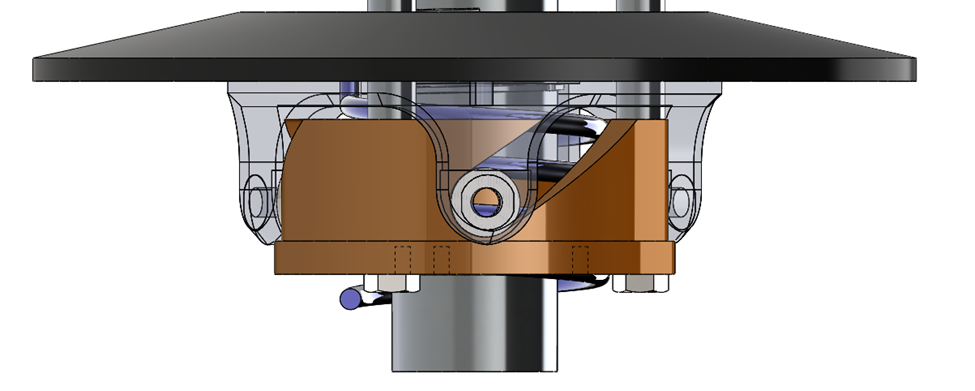
\includegraphics[scale=0.5]{secondaryCVTSideView.png}
          \caption{Secondary CVT Side View}
          \label{Fig_SecondaryCVTSideView}
      \end{minipage}
  \end{center}
\end{figure}

Note: The CVT that the McMaster Baja Team uses is slightly different from these figures but its mechanics are the same.


\subsubsection{Physical System Description} \label{sec_phySystDescrip}

The physical system of \progname{}, as shown in Figures 2-5,
includes the following elements:

\begin{itemize}

\item[PS1:] Fly weights
\begin{itemize}
  \item [PS1a:] mass ($m_{\text{fly}}$) in kg.
  \item [PS1b:] initial radius ($r_{\text{fly\_init}}$) in m.
  \item [PS1c:] final radius ($r_{\text{fly\_final}}$) in m. Might not be needed, just a limit
\end{itemize}

\item[PS2:] Primary spring

\begin{itemize}
  \item [PS2a:] spring constant ($k_{\text{prim}}$) in N/m.
  \item [PS2b:] pretension ($d_{\text{prim}}$) in m.
\end{itemize}

\item[PS3:] Primary ramp geometry function ($f_{\text{prim\_angle}}$)

\begin{itemize}
  \item [PS3a:] input distance ($d_{\text{prim\_in}}$) in m.
  \item [PS3b:] output angle ($\theta_{\text{prim\_out}}$) in radians.
\end{itemize}

\item[PS3:] Primary ramp height function ($f_{\text{prim\_height}}$)

\begin{itemize}
  \item [PS3a:] input distance ($d_{\text{prim\_in}}$) in m.
  \item [PS3c:] output height ($h_{\text{prim\_out}}$) in m.
\end{itemize}

\item[PS4:] Secondary spring

\begin{itemize}
  \item [PS4a:] compression spring constant ($k_{\text{sec\_comp}}$) in N/m.
  \item [PS4b:] torsional spring rate ($k_{\text{sec\_tor}}$) in Nm/rad.
  \item [PS4c:] pretension ($d_{\text{sec}}$) in m.
\end{itemize}

\item[PS5:] Secondary ramp geometry function ($f_{\text{sec}}$)

\begin{itemize}
  \item [PS5a:] input distance ($d_{\text{sec\_in}}$) in m.
  \item [PS5b:] output angle ($\theta_{\text{sec\_out}}$) in radians.
\end{itemize}

\item[PS6:] Weight

\begin{itemize}
  \item [PS6a:] driver weight ($m_{\text{driver}}$) in kg.
  \item [PS6b:] car weight ($m_{\text{car}}$) in kg.
\end{itemize}

\item[PS7:] Engine torque function ($f_{\text{engine}}$)

\begin{itemize}
  \item [PS7a:] input angular velocity ($\omega_{\text{engine}}$) in rad/s.
  \item [PS7b:] output torque ($T_{\text{engine}}$) in Nm.
\end{itemize}

\item[PS8:] Belt

\begin{itemize}
  \item [PS8a:] angle with sheave ($\theta_{\text{belt}}$). I think this does not need to exist, it matches the sheave angle?
  \item [PS8b:] friction coefficient ($\mu_{\text{belt}}$), unitless.
\end{itemize}

\item[PS9:] Total reduction

\begin{itemize}
  \item [PS9a:] gearbox reduction ratio ($r_{\text{gearbox}}$), unitless.
  \item [PS9b:] wheel radius ($r_{\text{wheel}}$) in m.
\end{itemize}

\item[PS10:] Coefficient of air resistance ($\mu_{\text{air}}$), unitless.

\item[PS11:] Center to Center distance ($d_{\text{center}}$) in m.

\item[PS12:] Angle on Incline ($\theta_{\text{incline}}$) in radians.

\item[PS13:] Secondary Ramp Radius ($r_{\text{sec\_ramp}}$) in m.

\item[PS14:] Traction ($\mu_{\text{traction}}$), unitless.

\end{itemize}
We might also want belt length, belt width, belt weight?, other properties

\subsubsection{Goal Statements}

\begin{itemize}

\item[GS\refstepcounter{goalnum}\thegoalnum \label{GS1}:]  Simulates the kinematics of the vehicle
\item[GS\refstepcounter{goalnum}\thegoalnum \label{GS2}:]  Simulates the output of the engine
\item[GS\refstepcounter{goalnum}\thegoalnum \label{GS3}:]  Simulates the CVT system over time

\end{itemize}

\subsection{Solution Characteristics Specification}

\plt{This section specifies the information in the solution domain of the system
  to be developed. This section is intended to express what is required in
  such a way that analysts and stakeholders get a clear picture, and the
  latter will accept it. The purpose of this section is to reduce the problem
  into one expressed in mathematical terms. Mathematical expertise is used to
  extract the essentials from the underlying physical description of the
  problem, and to collect and substantiate all physical data pertinent to the
  problem.}

\plt{This section presents the solution characteristics by successively refining
  models.  It starts with the abstract/general Theoretical Models (TMs) and
  refines them to the concrete/specific Instance Models (IMs).  If necessary
  there are intermediate refinements to General Definitions (GDs).  All of these
  refinements can potentially use Assumptions (A) and Data Definitions (DD).
  TMs are refined to create new models, that are called GMs or IMs. DDs are not
  refined; they are just used. GDs and IMs are derived, or refined, from other
  models. DDs are not derived; they are just given. TMs are also just given, but
  they are refined, not used.  If a potential DD includes a derivation, then
  that means it is refining other models, which would make it a GD or an IM.}

\plt{The above makes a distinction between ``refined'' and ``used.'' A model is
  refined to another model if it is changed by the refinement. When we change a
  general 3D equation to a 2D equation, we are making a refinement, by applying
  the assumption that the third dimension does not matter. If we use a
  definition, like the definition of density, we aren't refining, or changing
  that definition, we are just using it.}

\plt{The same information can be a TM in one problem and a DD in another.  It is
  about how the information is used.  In one problem the definition of
  acceleration can be a TM, in another it would be a DD.}

\plt{There is repetition between the information given in the different chunks
  (TM, GDs etc) with other information in the document.  For instance, the
  meaning of the symbols, the units etc are repeated.  This is so that the
  chunks can stand on their own when being read by a reviewer/user.  It also
  facilitates reuse of the models in a different context.}

\noindent \plt{The relationships between the parts of the document are show in
  the following figure.  In this diagram ``may ref'' has the same role as
  ``uses'' above.  The figure adds ``Likely Changes,'' which are able to
  reference (use) Assumptions.}

\begin{figure}[H]
  \includegraphics[scale=0.9]{RelationsBetweenTM_GD_IM_DD_A.pdf}
\end{figure}

The instance models that govern \progname{} are presented in
Subsection~\ref{sec_instance}.  The information to understand the meaning of the
instance models and their derivation is also presented, so that the instance
models can be verified.

\subsubsection{Types}

N/A

\subsubsection{Scope Decisions}

N/A
\subsubsection{Modelling Decisions}

N/A

\subsubsection{Assumptions} \label{sec_assumpt}

\begin{itemize}

\item[A\refstepcounter{assumpnum}\theassumpnum \label{A_1}:]
\textbf{Temperature variations} Ignore the effect of temperature on the material properties, excluding the belt.

\item[A\refstepcounter{assumpnum}\theassumpnum \label{A_2}:]
\textbf{negligible Gravitational Influence}: The orientation of the CVT system and gravitational effects are considered negligible due to the high rotational speeds involved in the system's operation.

\item[A\refstepcounter{assumpnum}\theassumpnum \label{A_3}:]
\textbf{Elasticity of Belts}: Elasticity of belts are assumed negligible, and the components are considered ideally rigid under normal operating conditions.

\item[A\refstepcounter{assumpnum}\theassumpnum \label{A_4}:]
\textbf{Vibrational Effects}: Vibrational effects from the vehicle or external environment are assumed to be minimal and are not factored into the transmission’s operation in this model.

\item[A\refstepcounter{assumpnum}\theassumpnum \label{A_5}:]
\textbf{Wear and Tear}: Component wear over time, including belt/chain wear and pulley degradation, is assumed negligible in the short-term operational model.

\item[A\refstepcounter{assumpnum}\theassumpnum \label{A_6}:]
\textbf{Frictional Losses in Non-critical Components}: Frictional losses in non-critical components (e.g., bearings, shafts) are assumed negligible, focusing only on friction relevant to the CVT system's core mechanics.

\item[A\refstepcounter{assumpnum}\theassumpnum \label{A_7}:]
\textbf{Engine Behavior Assumption:} The engine is modeled to operate at full throttle with consistent power curves and peak performance, maintaining a uniform response throughout the analysis. Load feedback will be integrated to adjust RPM and power output as necessary.
\end{itemize}

\subsubsection{Theoretical Models}\label{sec_theoretical}

\plt{Theoretical models are sets of abstract mathematical equations or axioms
  for solving the problem described in Section ``Physical System Description''
  (Section~\ref{sec_phySystDescrip}). Examples of theoretical models are
  physical laws, constitutive equations, relevant conversion factors, etc.}

\plt{Optionally the theory section could be divided into subsections to provide more structure and improve understandability and reusability.  Potential subsections include the following: Context theories, background theories, helper theories, generic theories, problem specific theories, final theories and rationale theories.}

This section focuses on the general equations and laws that \progname{} is based
on.  \plt{Modify the examples below for your problem, and add additional models
  as appropriate.}

\subsubsection*{General Theories}
This portion will specify the existing theories that are used in the development of the CVT simulation tool.

\noindent
\deftheory
{TM:HL}% #2 refname of theory
{Hookes Law}% #3 label
{$F = k \Delta x$}% #4 equation
{F is the force (N)\\
  k is the spring constant (N/m)\\
  $\Delta x$ is the displacement (m)\\}% #5 description
{In the context of this project Hookes law is used in both a torsional and linear way.}% #6 Notes
{\url{https://www.britannica.com/science/Hookes-law}}% #7 Source
{}% #8 Referenced by
{None}% #9 Preconditions
{}% #1 derivation - not applicable by default

~\newline

\noindent
\deftheory
{TM:CF}% #2 refname of theory
{Centrifugal Force}% #3 label
{$F_c = m \omega^2 r$}% #4 equation
{F is the force (N) \\
  m is the mass (kg)\\
  $\omega$ is the angular velocity (rad/s)\\
  r is the radius (m)\\}% #5 description
{None.}% #6 Notes
{\url{https://www.omnicalculator.com/physics/centrifugal-force}}% #7 Source
{}% #8 Referenced by
{None}% #9 Preconditions
{}% #1 derivation - not applicable by default

~\newline

\noindent
\deftheory
{TM:AR}% #2 refname of theory
{Air Resistance}% #3 label
{$F_d = \frac{1}{2} \rho v^2 C_d A$}% #4 equation
{F is the force (N)\\
  $\rho$ is the density of the fluid (kg/m$^3$)\\
  v is the velocity of the object (m/s)\\
  $C_d$ is the drag coefficient\\
  A is the cross-sectional area of the object (m$^2$)\\}% #5 description
{None.}% #6 Notes
{\url{https://softschools.com/formulas/physics/air_resistance_formula/85/}}% #7 Source
{}% #8 Referenced by
{None}% #9 Preconditions
{}% #1 derivation - not applicable by default

~\newline

\noindent
\deftheory
{TM:ET} % #2 refname of theory
{Engine Torque} % #3 label
{$\tau = \frac{P}{\omega}$} % #4 equation
{$\tau$ is the torque (N-m)\\
  P is the power (W)\\
  $\omega$ is the angular velocity (rad/s)\\}% #5 description
{None.}% #6 Notes
{\url{https://powertestdyno.com/how-to-calculate-horsepower/}}% #7 Source
{}% #8 Referenced by
{None}% #9 Preconditions
{}% #1 derivation - not applicable by default

~\newline

\noindent
\deftheory
{TM:GR}% #2 refname of theory
{Secondary Torque}% #3 label
{$\tau_{\text{output}} = \tau_{\text{input}} \times \text{gear reduction}$}% #4 equation
{$\tau_{\text{output}}$ is the output torque (N-m)\\
  $\tau_{\text{input}}$ is the input torque (N-m)\\}% #5 description
{None.}% #6 Notes
{}% #7 Source
{}% #8 Referenced by
{None}% #9 Preconditions
{}% #1 derivation - not applicable by default

~\newline

\noindent
\deftheory
{TM:FR}% #2 refname of theory
{Friction Formula}% #3 label
{$F_f = \mu F_n$}% #4 equation
{$\mu_{\text{effective}}$ is the effective coefficient of friction\\
  $\mu_{\text{nominal}}$ is the nominal coefficient of friction\\
  $\phi$ is the angle of wrap of the belt (radians)\\}% #5 description
{None.}% #6 Notes
{}% #7 Source
{}% #8 Referenced by
{None}% #9 Preconditions
{}% #1 derivation - not applicable by default

\noindent
\deftheory
{TM:DE}% #2 refname of theory
{Density}% #3 label
{$\rho = \frac{m}{V}$}% #4 equation
{$\rho$ is the density (kg/m$^3$)\\
  m is the mass (kg)\\
  V is the volume (m$^3$)\\}% #5 description
{None.}% #6 Notes
{\url{https://www.britannica.com/science/density-physics}}% #7 Source
{}% #8 Referenced by
{None}% #9 Preconditions
{}% #1 derivation - not applicable by default

~\newline

\noindent
\deftheory
{TM:CE}% #2 refname of theory
{Capstan Equation}% #3 label
{$T_1 = T_2 e^{\mu \theta}$}% #4 equation
{$T_1$ is the tension on the first side of the belt (N)\\
  $T_2$ is the tension on the second side of the belt (N)\\
  $\mu$ is the coefficient of friction\\
  $\theta$ is the angle of wrap of the belt (radians)\\}% #5 description
{None.}% #6 Notes
{\url{https://hackaday.com/2021/01/26/cable-mechanism-maths-designing-against-the-capstan-equation/}}% #7 Source
{}% #8 Referenced by
{None}% #9 Preconditions
{}% #1 derivation - not applicable by default

~\newline

\noindent
\deftheory
{TM:N2}% #2 refname of theory
{Newtons 2nd Law}% #3 label
{$F = ma$}% #4 equation
{  F is the force (N)\\
  m is the mass (kg)\\
  a is the acceleration (m/s$^2$)\\}% #5 description
{Newtons 2nd law is used repeatedly in several Instance models}% #6 Notes
{\url{https://www.physicsclassroom.com/class/newtlaws/lesson-3/newton-s-second-law}}% #7 Source
{}% #8 Referenced by
{None}% #9 Preconditions
{}% #1 derivation - not applicable by default

\subsubsection*{Helper Theories}
This portion will define auxiliary theories to aid in further derivation below.


Add here stuff like:
- in: shift distance, out: radius of pulley
- in: shift distance, out: angle of ramp
- in: shift distance, out: angle of helix

\plt{``Ref.\ By'' is used repeatedly with the different types of information.
  This stands for Referenced By.  It means that the models, definitions and
  assumptions listed reference the current model, definition or assumption.
  This information is given for traceability.  Ref. By provides a pointer in the
  opposite direction to what we commonly do.  You still need to have a reference
  in the other direction pointing to the current model, definition or
  assumption.  As an example, if TM1 is referenced by GD2, that means that GD2 will
  explicitly include a reference to TM1.}

~\newline

\subsubsection{General Definitions}\label{sec_gendef}

We do not have any general definitions at this time.

\subsubsection{Data Definitions}\label{sec_datadef}

\plt{The Data Definitions are definitions of symbols and equations that are
  given for the problem.  They are not derived; they are simply used by other
  models.  For instance, if a problem depends on density, there may be a data
  definition for the equation defining density.  The DDs are given information
  that you can use in your other modules.}

\plt{All Data Definitions should be used (referenced) by at least one other
  model.}

This section collects and defines all the data needed to build the instance
models. The dimension of each quantity is also given.  \plt{Modify the examples
  below for your problem, and add additional definitions as appropriate.}

data definitions so far, more to be added later
\begin {itemize}
\item velocity
\item acceleration
\item torque
\item friction
\item rpm
\end {itemize}

~\newline

\noindent
\begin{minipage}{\textwidth}
\renewcommand*{\arraystretch}{1.5}
\begin{tabular}{| p{\colAwidth} | p{\colBwidth}|}
\hline
\rowcolor[gray]{0.9}
Number& DD\refstepcounter{datadefnum}\thedatadefnum \label{FluxCoil}\\
\hline
Label& \bf Heat flux out of coil\\
\hline
Symbol &$q_C$\\
\hline
% Units& $Mt^{-3}$\\
% \hline
  SI Units & \si{\watt\per\square\metre}\\
  \hline
  Equation&$q_C(t) = h_C (T_C - T_W(t))$, over area $A_C$\\
  \hline
  Description & 
                $T_C$ is the temperature of the coil (\si{\celsius}).  $T_W$ is the temperature of the water (\si{\celsius}).  
                The heat flux out of the coil, $q_C$ (\si{\watt\per\square\metre}), is found by
                assuming that Newton's Law 
                of Cooling applies (\aref{A_Newt_coil}).  This law (\dref{NL}) is used on the surface of
                the coil, which has area $A_C$ (\si{\square\metre}) and heat 
                transfer coefficient $h_C$
                (\si{\watt\per\square\metre\per\celsius}).  This equation
                assumes that the temperature of the coil is constant over time (\aref{A_tcoil}) and that it does not vary along the length
                of the coil (\aref{A_tlcoil}).
  \\
  \hline
  Sources& Citation here \\
  \hline
  Ref.\ By & \iref{ewat}\\
  \hline
\end{tabular}
\end{minipage}\\

\subsubsection{Data Types}\label{sec_datatypes}

N/A

\subsubsection{Instance Models} \label{sec_instance}    

This section transforms the problem defined in Section~\ref{Sec_pd} into 
one which is expressed in mathematical terms. It uses concrete symbols defined 
in Section~\ref{sec_datadef} to replace the abstract symbols in the models 
identified in Sections~\ref{sec_theoretical} and~\ref{sec_gendef}.
{\newline}

{\noindent}The goal statment GS\ref{GS1} are solved by Instance Models \ref{inst:1}, \ref{inst:2} and \ref{inst:3}\\
The goal statement GS\ref{GS3} are solved by Instance Models \ref{inst:4} and \ref{inst:5}\\
  \definstance
  {Acceleration}
  {$r_{\text{gear}}, r_{\text{wheel}}, \rho, C_D, A, \theta, T_{\text{CVT}}, C_{\text{rr}}, m_v, m_d$}
  {$a = \frac{\left( \frac{T_{\text{CVT}}}{r_{\text{gear}} + r_{\text{wheel}}} \right) - (C_{\text{rr}} F_g \sin(\theta)) - \left( \frac{1}{2} \rho v^2 C_D A \right) - (F_g \cos(\theta))}{m_v + m_d}$}
  {acceleration a}
  {$r_{\text{gear}}$ is the radius of the gear (m)\\
  & $r_{\text{wheel}}$ is the radius of the wheel (m)\\
  & $\rho$ is the density of the fluid (kg/m$^3$)\\
  & $C_D$ is the drag coefficient\\
  & A is the cross-sectional area of the object (m$^2$)\\
  & $\theta$ is the angle of incline ($\theta$)\\
  & $T_{\text{CVT}}$ is the torque transferred to the wheel (N-m)\\
  & $C_{\text{rr}}$ is the coefficient of rolling resistance\\
  & $m_v$ is the mass of the vehicle (kg)\\
  & $m_d$ is the mass of the driver(kg)}
  {-}
  
  
  \subsubsection*{Derivation of acceleration}
  The acceleration of the vehicle is derived as such: \\
  $T_W - R_r - F_D - F_g \cos(\theta) = ma$\\
  Where $T_W$ is the torque of the wheel, $R_r$ is the rolling resistance, $F_D$ is the drag force, $F_g$ is the gravitational force, and $m$ is the mass of the vehicle.\\
  $T_W = \frac{T_{\text{CVT}}}{r_{\text{gear}} + r_{\text{wheel}}}$\\
  $R_r = C_{\text{rr}} F_g \sin(\theta)$\\
  $F_D = \frac{1}{2} \rho v^2 C_D A$\\
  $m = m_v + m_d$\\
  Substitute the above equations into the original equation to get the final equation for acceleration.\\
  $a = \frac{\left( \frac{T_{\text{CVT}}}{r_{\text{gear}} + r_{\text{wheel}}} \right) - (C_{\text{rr}} F_g \sin(\theta)) - \left( \frac{1}{2} \rho v^2 C_D A \right) - (F_g \cos(\theta))}{m_v + m_d}$

\definstance
{Velocity}
{$a(t)$}
{$v(t) = \int a(t) dt$}
{$v(t)$}
{$a(t)$ is the function of acceleration over time}
{-}

\definstance
{Distance}
{$v(t)$}
{$d(t) = \int v(t) dt$}
{$d(t)$}
{$v(t)$ is the function of velocity over time}
{-}

\definstance
{Primary Clamping Force}
{$m$, $r_{\text{flyi}}$, $h_{\text{prim}}$, $F_{\text{prim}}(d_{\text{shift}})$, $K_{\text{prim}}$, $d_{\text{prc}}$, $d_{\text{shift}}$} % Input
{$F_{FW} - F_S = m (r_{\text{flyi}} + F_{\text{primHeight}}({d_\text{{shift}}})) \cdot \tan(F_{\text{prim}}(d_{\text{shift}})) + K_{\text{prim}} (d_{\text{prc}} + d_{\text{shift}})$} % 
{$F_{FW} - F_S$ where $F_{FW}$ is the flywheel force and $F_S$ is the spring force, representing the total primary clamping force.} % Output
{$m$: Mass of the system. \\ 
  &$r_{\text{flyi}}$: Radius related to the flywheel. \\ 
  &$F_{\text{primHeight}}(d_{\text{shift}})$: Function that represents the height of the primary system. \\
  &$F_{\text{prim}}(d_{\text{shift}})$: Primary function that represents the force dependent on the shifting distance. \\ 
  &$K_{\text{prim}}$: Stiffness or coefficient related to the primary system. \\ 
  &$d_{\text{prc}}$: Pre-compression or pre-load distance. \\ 
  &$d_{\text{shift}}$: Displacement or shift in the system.} % Description
{} % Sources
{-}

\subsubsection*{Derivation of Primary Clamping Force}
The flywheel force is derived as such: \\
$F_{FW} = m r \omega^2 \cdot \tan(F_{\text{prim}}(d_{\text{shift}}))$\\
Where $r \omega^2$ can repersented by $r_{\text{flyi}}+h_{\text{prim}}$\\
Then $F_{FW}$ becomes $m (r_{\text{flyi}} + h_{\text{prim}}) \cdot \tan(F_{\text{prim}}(d_{\text{shift}}))$\\
{\newline}
The spring force is derived as such: \\
$-F_S$ = $+ K_{\text{prim}} (d_{\text{prc}} + d_{\text{shift}})$\\
{\newline}
Combine those two forces to get the total primary clamping force.\\
$F_{FW} - F_S = m (r_{\text{flyi}} + h_{\text{prim}}) \cdot \tan(F_{\text{prim}}(d_{\text{shift}})) + K_{\text{prim}} (d_{\text{prc}} + d_{\text{shift}})$ 


\definstance
{Secondary Clamping Force}
{$K_e$, $\theta_{\text{sec}}$, $\theta_{\text{shift}}$, $r_{\text{secramp}}$, $f_{\text{sec}}(d_{\text{shift}})$, $K_c$, $\delta_{\text{sec}}$, $d_{\text{shift}}$} % Input
{$F_S + F_H = \frac{K_e (\theta_{\text{sec}} + \theta_{\text{shift}}) + T_{eng} CVT_{ratio}}{2 \cdot r_{\text{secramp}} \cdot \tan(f_{\text{sec}}(d_{\text{shift}}))} + K_c (\delta_{\text{sec}} + d_{\text{shift}})$} % 
{$F_s + F_H$ where $F_S$ is spring clamping force and $F_H$ is the helix clamping force added together are the total the secondary clamping force } % Output
{$K_e$: Stiffness or spring constant related to elastic deformation. \\
  &$\theta_{\text{sec}}$: Secondary angle or rotational position. \\
  &$\theta_{\text{shift}}$: Shift in the secondary angle. \\
  &$r_{\text{secramp}}$: Radius or ramp characteristic related to the secondary system. \\
  &$f_{\text{sec}}(d_{\text{shift}})$: Function representing the force as a function of the secondary displacement or shift. \\
  &$K_c$: Stiffness or coefficient related to a damping or correction factor. \\
  &$\delta_{\text{sec}}$: Secondary deflection or displacement variable. \\
  &$d_{\text{shift}}$: Displacement or shift in the system.\\
  &$T_{eng}$: Torque of the engine. \\
  &$CVT_{ratio}$: Ratio of the CVT system.
} % Description
{} % Sources
{-}

\subsubsection*{Derivation of Secondary Clamping Force}
The spring force is derived as such: \\
$F_S = \frac{K_e (\theta_{\text{sec}} + \theta_{\text{shift}})}{2 \cdot r_{\text{secramp}} \cdot \tan(f_{\text{sec}}(d_{\text{shift}}))} + K_c (\delta_{\text{sec}} + d_{\text{shift}})$\\
{\newline}
The helix force is derived as such: \\
$F_H = \frac{T_{eng} CVT_{ratio}}{2 \cdot r_{\text{secramp}} \cdot \tan(f_{\text{sec}}(d_{\text{shift}}))}$\\
{\newline}
Combine those two forces to get the total secondary clamping force.\\
$F_S + F_H = \frac{K_e (\theta_{\text{sec}} + \theta_{\text{shift}}) + T_{eng} CVT_{ratio}}{2 \cdot r_{\text{secramp}} \cdot \tan(f_{\text{sec}}(d_{\text{shift}}))} + K_c (\delta_{\text{sec}} + d_{\text{shift}})$


\definstance
{CVT Ratio}
{} % Input
{} % Output
{} % Description
{} % Sources
{} % Citation
{-}

\definstance
{Torque Transferred}
{} % Input
{} % Output
{} % Description
{} % Sources
{} % Citation
{-}

\definstance
{RPM and Torque of Engine}
{} % Input
{} % Output
{} % Description
{} % Sources
{} % Citation
{-}

\subsubsection{Input Data Constraints} \label{sec_DataConstraints}    

Table~\ref{TblInputVar} shows the data constraints on the input output
variables.  The column for physical constraints gives the physical limitations
on the range of values that can be taken by the variable.  The column for
software constraints restricts the range of inputs to reasonable values.  The
software constraints will be helpful in the design stage for picking suitable
algorithms.  The constraints are conservative, to give the user of the model the
flexibility to experiment with unusual situations.  The column of typical values
is intended to provide a feel for a common scenario.  The uncertainty column
provides an estimate of the confidence with which the physical quantities can be
measured.  This information would be part of the input if one were performing an
uncertainty quantification exercise.

The specification parameters in Table~\ref{TblInputVar} are listed in
Table~\ref{TblSpecParams}.

\begin{table}[!h]
  \caption{Input Variables} \label{TblInputVar}
  \renewcommand{\arraystretch}{1.2}
\noindent \begin{longtable*}{l l l l c} 
  \toprule
  \textbf{Var} & \textbf{Physical Constraints} & \textbf{Software Constraints} &
                             \textbf{Typical Value} & \textbf{Uncertainty}\\
  \midrule 
  $L$ & $L > 0$ & $L_{\text{min}} \leq L \leq L_{\text{max}}$ & 1.5 \si[per-mode=symbol] {\metre} & 10\%\\
  % params
  $m_{fly}$ & $0 \leq m_{fly}$ & $m_{fly} \leq 1$ & 0.2 kg\\
  $\omega_{engine}$ & $0 \leq \omega_{engine}$ & $\omega_{engine} \leq \omega_\text{max}$ & 400 rad/s\\
  % Cannot shift more than width of belt
  $d_{shift}$ & $0 \leq d_{shift} \leq w_{belt}$ & & 0.1 m\\
  % Angle of ramp cannot exceed 90 degrees
  $\theta_{prim\_out}$ & $0 \leq \theta_{prim\_out} \leq \frac{\pi}{2}$ & & $\frac{\pi}{4}$ rad\\
  % Pretension
  $d_{\text{prim}}$ & $0 \leq d_{\text{prim}} \leq d_\text{max\_prim\_pre}$ & & 0.1 m\\
  $d_{\text{sec}}$ & $0 \leq d_{\text{sec}} \leq d_\text{max\_sec\_pre}$ & & 0.1 rad\\
  % Weight
  $m_{\text{driver}}$ & $0 \leq m_{\text{driver}}$ & $ m_{\text{driver}} \leq m_\text{max\_human}$ & 75 kg\\
  $m_{\text{car}}$ & $0 \leq m_{\text{car}}$ & $m_{\text{car}} \leq m_\text{max\_car}$ & 225 kg\\
  % Spring rate
  $k_{\text{prim}}$ & $0 \leq k_{\text{prim}}$ & $k_{\text{prim}} \leq k_\text{max\_comp\_spring}$ & 100 N/m\\
  $k_{\text{sec\_comp}}$ & $0 \leq k_{\text{sec\_comp}}$ & $k_{\text{sec\_comp}} \leq k_\text{max\_comp\_spring}$ & 100 N/m\\
  $k_{\text{sec\_tor}}$ & $0 \leq k_{\text{sec\_tor}}$ & $k_{\text{sec\_tor}} \leq k_\text{max\_tor\_spring}$ & 50 Nm/rad\\
  \bottomrule
\end{longtable*}
\end{table}

\noindent 
\begin{description}
\item[(*)] \plt{you might need to add some notes or clarifications}
\end{description}

\begin{table}[!h]
\caption{Specification Parameter Values} \label{TblSpecParams}
\renewcommand{\arraystretch}{1.2}
\noindent \begin{longtable*}{l l} 
  \toprule
  \textbf{Var} & \textbf{Value} \\
  \midrule 
  $L_\text{min}$ & 0.1 \si{\metre}\\
  $\omega_\text{max}$ & 600 rad/s\\
  $w_\text{belt}$ & UNKNOWN, see belt spec m\\
  $d_\text{max\_prim\_pre}$ & UNKNOWN, see CAD m\\
  $d_\text{max\_sec\_pre}$ & UNKNOWN, see CAD rad\\
  $m_\text{max\_human}$ & 200 kg\\
  $m_\text{max\_car}$ & 350 kg\\
  $k_\text{max\_comp\_spring}$ & 1000 N/m\\
  $k_\text{max\_tor\_spring}$ & 750 Nm/rad\\
  $v_\text{max}$ & UNKNOWN, do gear calcs m/s\\
  $f_\text{belt\_max}$ & UNKNOWN, see belt spec N\\
  \bottomrule
\end{longtable*}
\end{table}

\subsubsection{Properties of a Correct Solution} \label{sec_CorrectSolution}

\noindent
A correct solution must exhibit \plt{fill in the details}.  \plt{These
  properties are in addition to the stated requirements.  There is no need to
  repeat the requirements here.  These additional properties may not exist for
  every problem.  Examples include conservation laws (like conservation of
  energy or mass) and known constraints on outputs, which are usually summarized
  in tabular form.  A sample table is shown in Table~\ref{TblOutputVar}}

\begin{table}[!h]
\caption{Output Variables} \label{TblOutputVar}
\renewcommand{\arraystretch}{1.2}
\noindent \begin{longtable*}{l l l} 
  \toprule
  \textbf{Var} & \textbf{Physical Constraints} & \textbf{unit}\\
  \midrule 
  $T_W$ & $T_\text{init} \leq T_W \leq T_C$ (by~\aref{A_charge}) & unitless\\
  $v(t)$ & $0 \leq v(t) \leq v_\text{max}$& m/s\\
  $\text{Sum of clamping forces}$ & $\text{Clamp} \leq f_\text{belt\_max}$ & N \\
  \bottomrule
\end{longtable*}
\end{table}

\plt{This section is not for test cases or techniques for verification and
  validation.  Those topics will be addressed in the Verification and Validation
  plan.}

\section{Requirements}

This section provides the functional requirements, the business tasks that the
software is expected to complete, and the nonfunctional requirements, the
qualities that the software is expected to exhibit.

\subsection{Functional Requirements}

\noindent \begin{itemize}

\item[R\refstepcounter{reqnum}\thereqnum \label{R_Inputs}:] The system shall simulate the behavior of the McMaster Baja Team's Continuous Variable Transmission(CVT) using mathematical models.

\item[R\refstepcounter{reqnum}\thereqnum \label{R_Inputs}:] The system shall allow users to adjust the following CVT tunning parameters: primary weight, primary ramp geometry, primary spring rate, primary spring Pretension, secondary helix geometry, secondary spring rate, secondary spring pretension. 

\item[R\refstepcounter{reqnum}\thereqnum \label{R_Inputs}:] The system shall allow users to adjust vehicle and driver weight, traction and angle of incline in addition to the CVT tuning parameters.

\item[R\refstepcounter{reqnum}\thereqnum \label{R_Inputs}:] The system shall provide users with an interface to input tuning parameters.

\item[R\refstepcounter{reqnum}\thereqnum \label{R_Inputs}:] The system shall display graphs of simulation output based on the user inputted tuning parameters.

\item[R\refstepcounter{reqnum}\thereqnum \label{R_Inputs}:] The system shall allow users to compare results of simulations with different CVT tuning parameters.

\item[R\refstepcounter{reqnum}\thereqnum \label{R_Inputs}:] The system shall calculate the CVT ratio, clamping force, RPM, torque and belt slippage as functions of time. Combined with engine input, the system shall calculate distance, speed and acceleration as functions of time.

\item[R\refstepcounter{reqnum}\thereqnum \label{R_Inputs}:] The system shall allow users to export outputted simulated graphical data.

\item[R\refstepcounter{reqnum}\thereqnum \label{R_Inputs}:] The system shall allow users to access the application through the use of a personal computer or laptop.

\item[R\refstepcounter{reqnum}\thereqnum \label{R_Inputs}:] The system shall be compatible with Windows, MacOS and Linux.
\end{itemize}

\subsection{Nonfunctional Requirements}

\noindent \begin{itemize}

\item[NFR\refstepcounter{nfrnum}\thenfrnum \label{NFR_Accuracy}:]\textbf{Accuracy} The system shall achieve an accuracy of at least 95 \% in correctly predicting CVT outputs.
\item[NFR\refstepcounter{nfrnum}\thenfrnum \label{NFR_Usability}:] \textbf{Usability} 85 \% of a representative user group shall be able to successively input CVT parameters and receive CVT outputs on their first use.
\item[NFR\refstepcounter{nfrnum}\thenfrnum \label{NFR_Maintainability}:]\textbf{Maintainability} If a likely change is made to the finished software, it will take at most 10 \% of the original development time, assuming the same development resources are available.
\item[NFR\refstepcounter{nfrnum}\thenfrnum \label{NFR_Verifiability}:] \textbf{Verifiability} The system shall output the resulting tunned CVT outputs which must able to be cross-verified against data available through the McMaster Baja Team with a consistency rate of 95 \%.
\item[NFR\refstepcounter{nfrnum}\thenfrnum \label{NFR_Understandability}:] \textbf{Understandability} The system shall be understood by at least 90 \% of a representative user group with no more than 15 minutes of initial training, as measured by assessing ability to generate and export tunned CVT output where users must score at least 90 \%
\item[NFR\refstepcounter{nfrnum}\thenfrnum \label{NFR_Reusability}:] \textbf{Reusability} The system's components shall be designed for reuse in the case the McMaster Baja team acquires a new CVT. These modifications should be made with minimal modifications, defined as requiring modification to less than 30 \% of the code to configure these changes.

\end{itemize}

\subsection{Rationale}

The assumptions made for the CVT (Continuously Variable Transmission) system model aim to simplify its dynamics, making it easier to analyze and develop a solution. 
A key assumption is the exclusion of temperature effects on material properties, aside from the belt, which allows for a more straightforward focus on the mechanics of the interactions (A1). 
The negligible influence of gravitational forces, further simplifies the problem by removing the need to eliminating the need to consider variations in position. 
Additionally, the elasticity of belts is considered insignificant, treating components as ideally rigid, allowing the development of a model without accounting for material deformations (A3). 
Vibrational effects from external sources are also assumed to be minimal, avoiding the complexity of vibration-induced disturbances in the transmission behavior (A4). 
Wear and tear of components, including the belt and pulley are disregarded for short-term operational modeling, allowing for an idealized performance assumption (A5). 
Frictional losses in non-critical components, are deemed negligible, allowing the focus to frictional effects that directly impact the CVT’s core mechanics (A6). 
Finally, the engine is assumed to operate at full throttle with consistent power delivery, simplifying the model by maintaining uniform engine behavior (A4).
These simplifications affect the process of formulating equations governing velocity, distance, primary clamping force, secondary clamping force, CVT Ratio, Torque transfer and RPM and Torque of the Engine(IM1-IM8)

\section{Likely Changes}    

\noindent \begin{itemize}

\item[LC\refstepcounter{lcnum}\thelcnum\label{LC_1}:] The effect of temperature on material properties might be included in the future, (A\ref{A_1})
\item[LC\refstepcounter{lcnum}\thelcnum\label{LC_2}:] The elasticity of the belt might be considered in the future, (A\ref{A_3})
\item[LC\refstepcounter{lcnum}\thelcnum\label{LC_3}:] Frictional losses in non-critical components might be considered in the future, (A\ref{A_6})
\item[LC\refstepcounter{lcnum}\thelcnum\label{LC_4}:] Some of the math models will most likely change as the design is refined.

\end{itemize}

\section{Unlikely Changes}    

None
\section{Traceability Matrices and Graphs}

The purpose of the traceability matrices is to provide easy references on what
has to be additionally modified if a certain component is changed.  Every time a
component is changed, the items in the column of that component that are marked
with an ``X'' may have to be modified as well.  Table~\ref{Table:trace} shows the
dependencies of theoretical models, general definitions, data definitions, and
instance models with each other. Table~\ref{Table:R_trace} shows the
dependencies of instance models, requirements, and data constraints on each
other. Table~\ref{Table:A_trace} shows the dependencies of theoretical models,
general definitions, data definitions, instance models, and likely changes on
the assumptions.

\plt{You will have to modify these tables for your problem.}

\plt{The traceability matrix is not generally symmetric.  If GD1 uses A1, that
  means that GD1's derivation or presentation requires invocation of A1.  A1
  does not use GD1.  A1 is ``used by'' GD1.}

\plt{The traceability matrix is challenging to maintain manually.  Please do
  your best.  In the future tools (like Drasil) will make this much easier.}

  \afterpage{
    \begin{landscape}
    \begin{table}[h!]
    \centering
    \begin{tabular}{|c|c|c|c|c|c|c|c|c|c|c|c|c|c|c|c|c|c|c|c|}
    \hline
      & \aref{A_OnlyThermalEnergy}& \aref{A_hcoeff}& \aref{A_mixed}& \aref{A_tpcm}& \aref{A_const_density}& \aref{A_const_C}& \aref{A_Newt_coil}& \aref{A_tcoil}& \aref{A_tlcoil}& \aref{A_Newt_pcm}& \aref{A_charge}& \aref{A_InitTemp}& \aref{A_OpRangePCM}& \aref{A_OpRange}& \aref{A_htank}& \aref{A_int_heat}& \aref{A_vpcm}& \aref{A_PCM_state}& \aref{A_Pressure} \\
    \hline
    \tref{T_COE}        & X& & & & & & & & & & & & & & & & & & \\ \hline
    \tref{T_SHE}        & & & & & & & & & & & & & & & & & & & \\ \hline
    \tref{T_LHE}        & & & & & & & & & & & & & & & & & & & \\ \hline
    \dref{NL}           & & X& & & & & & & & & & & & & & & & & \\ \hline
    \dref{ROCT}         & & & X& X& X& X& & & & & & & & & & & & & \\ \hline
    \ddref{FluxCoil}    & & & & & & & X& X& X& & & & & & & & & & \\ \hline
    \ddref{FluxPCM}     & & & X& X& & & & & & X& & & & & & & & & \\ \hline
    \ddref{D_HOF}       & & & & & & & & & & & & & & & & & & & \\ \hline
    \ddref{D_MF}        & & & & & & & & & & & & & & & & & & & \\ \hline
    \iref{ewat}         & & & & & & & & & & & X& X& & X& X& X& & & X \\ \hline
    \iref{epcm}         & & & & & & & & & & & & X& X& & & X& X& X& \\ \hline
    \iref{I_HWAT}       & & & & & & & & & & & & & & X& & & & & X \\ \hline
    \iref{I_HPCM}       & & & & & & & & & & & & & X& & & & & X & \\ \hline
    \lcref{LC_tpcm}     & & & & X& & & & & & & & & & & & & & & \\ \hline
    \lcref{LC_tcoil}    & & & & & & & & X& & & & & & & & & & & \\ \hline
    \lcref{LC_tlcoil}   & & & & & & & & & X& & & & & & & & & & \\ \hline
    \lcref{LC_charge}   & & & & & & & & & & & X& & & & & & & & \\ \hline
    \lcref{LC_InitTemp} & & & & & & & & & & & & X& & & & & & & \\ \hline
    \lcref{LC_htank}    & & & & & & & & & & & & & & & X& & & & \\
    \hline
    \end{tabular}
    \caption{Traceability Matrix Showing the Connections Between Assumptions and Other Items}
    \label{Table:A_trace}
    \end{table}
    \end{landscape}
    }

\afterpage{
\begin{landscape}
\begin{table}[h!]
\centering
\begin{tabular}{|c|c|c|c|c|c|c|c|}
\hline
	& \aref{A_1}& \aref{A_2}& \aref{A_3}& \aref{A_4}& \aref{A_5}& \aref{A_6}& \aref{A_7}\\
\hline
\tref{TM:HL}        & & & & & & & \\ \hline
\tref{TM:CF}        & & & & & & & \\ \hline
\tref{TM:AR}        & & & & & & & \\ \hline
\tref{TM:ET}        & & & & & & & \\ \hline
\tref{TM:GR}        & & & & & & & \\ \hline
\tref{TM:FR}        & & & & & & & \\ \hline
\tref{TM:DE}        & & & & & & & \\ \hline
\tref{TM:CE}        & & & & & & & \\ \hline
\tref{TM:N2}        & & & & & & & \\ \hline
\iref{inst:1}       & & & & & & & \\ \hline
\iref{inst:2}       & & & & & & & \\ \hline
\iref{inst:3}       & & & & & & & \\ \hline
\iref{inst:4}       & & & & & & & \\ \hline
\iref{inst:5}       & & & & & & & \\ \hline
\iref{inst:6}       & & & & & & & \\ \hline
\iref{inst:7}       & & & & & & & \\ \hline
\iref{inst:8}       & & & & & & & \\ \hline
\lcref{LC_1}        & & & & & & & \\ \hline
\lcref{LC_2}        & & & & & & & \\ \hline
\lcref{LC_3}        & & & & & & & \\ \hline
\lcref{LC_4}        & & & & & & & \\
\hline
\end{tabular}
\caption{Traceability Matrix Showing the Connections Between Assumptions and Other Items}
\label{Table:A_trace}
\end{table}
\end{landscape}
}


\begin{table}[h!]
  \centering
  \begin{tabular}{|c|c|c|c|c|c|c|c|c|c|c|c|c|c|c|c|c|c|c|c|c|c|c|c|}
  \hline        
    & \tref{T_COE}& \tref{T_SHE}& \tref{T_LHE}& \dref{NL}& \dref{ROCT} & \ddref{FluxCoil}& \ddref{FluxPCM} & \ddref{D_HOF}& \ddref{D_MF}& \iref{ewat}& \iref{epcm}& \iref{I_HWAT}& \iref{I_HPCM} \\
  \hline
  \tref{T_COE}     & & & & & & & & & & & & & \\ \hline
  \tref{T_SHE}     & & & X& & & & & & & & & & \\ \hline
  \tref{T_LHE}     & & & & & & & & & & & & & \\ \hline
  \dref{NL}        & & & & & & & & & & & & & \\ \hline
  \dref{ROCT}      & X& & & & & & & & & & & & \\ \hline
  \ddref{FluxCoil} & & & & X& & & & & & & & & \\ \hline
  \ddref{FluxPCM}  & & & & X& & & & & & & & & \\ \hline
  \ddref{D_HOF}    & & & & & & & & & & & & & \\ \hline
  \ddref{D_MF}     & & & & & & & & X& & & & & \\ \hline
  \iref{ewat}      & & & & & X& X& X& & & & X& & \\ \hline
  \iref{epcm}      & & & & & X& & X& & X& X& & & X \\ \hline
  \iref{I_HWAT}    & & X& & & & & & & & & & & \\ \hline
  \iref{I_HPCM}    & & X& X& & & & X& X& X& & X& & \\
  \hline
  \end{tabular}
  \caption{Traceability Matrix Showing the Connections Between Items of Different Sections}
  \label{Table:trace}
  \end{table}

\begin{table}[h!]
\centering
\begin{tabular}{|c|c|c|c|c|c|c|c|c|c|c|c|c|c|c|c|c|c|c|c|c|c|}
\hline        
	& \tref{TM:HL}& \tref{TM:CF}& \tref{TM:AR}& \tref{TM:ET}& \tref{TM:GR}& \tref{TM:FR}& \tref{TM:DE}& \tref{TM:CE}& \tref{TM:N2}& \iref{inst:1}& \iref{inst:2}& \iref{inst:3}& \iref{inst:4}& \iref{inst:5}& \iref{inst:6}& \iref{inst:7}& \iref{inst:8}& \\
\hline
\tref{TM:HL}        & & & & & & & & & & & & & & & & & \\ \hline
\tref{TM:CF}        & & & & & & & & & & & & & & & & & \\ \hline
\tref{TM:AR}        & & & & & & & & & & & & & & & & & \\ \hline
\tref{TM:ET}        & & & & & & & & & & & & & & & & & \\ \hline
\tref{TM:GR}        & & & & & & & & & & & & & & & & & \\ \hline
\tref{TM:FR}        & & & & & & & & & & & & & & & & & \\ \hline
\tref{TM:DE}        & & & & & & & & & & & & & & & & & \\ \hline
\tref{TM:CE}        & & & & & & & & & & & & & & & & & \\ \hline
\tref{TM:N2}        & & & & & & & & & & & & & & & & & \\ \hline
\iref{inst:1}       & & & & & & & & & & & & & & & & & \\ \hline
\iref{inst:2}       & & & & & & & & & & & & & & & & & \\ \hline
\iref{inst:3}       & & & & & & & & & & & & & & & & & \\ \hline
\iref{inst:4}       & & & & & & & & & & & & & & & & & \\ \hline
\iref{inst:5}       & & & & & & & & & & & & & & & & & \\ \hline
\iref{inst:6}       & & & & & & & & & & & & & & & & & \\ \hline
\iref{inst:7}       & & & & & & & & & & & & & & & & & \\ \hline
\iref{inst:8}       & & & & & & & & & & & & & & & & & \\
\hline
\end{tabular}
\caption{Traceability Matrix Showing the Connections Between Items of Different Sections}
\label{Table:trace}
\end{table}

\begin{table}[h!]
\centering
\begin{tabular}{|c|c|c|c|c|c|c|c|}
\hline
	& \iref{ewat}& \iref{epcm}& \iref{I_HWAT}& \iref{I_HPCM}& \ref{sec_DataConstraints}& \rref{R_RawInputs}& \rref{R_MassInputs} \\
\hline
\iref{ewat}            & & X& & & & X& X \\ \hline
\iref{epcm}            & X& & & X& & X& X \\ \hline
\iref{I_HWAT}          & & & & & & X& X \\ \hline
\iref{I_HPCM}          & & X& & & & X& X \\ \hline
\rref{R_RawInputs}     & & & & & & & \\ \hline
\rref{R_MassInputs}    & & & & & & X& \\ \hline
\rref{R_CheckInputs}   & & & & & X& & \\ \hline
\rref{R_OutputInputs}  & X& X& & & & X& X \\ \hline
\rref{R_TempWater}     & X& & & & & & \\ \hline 
\rref{R_TempPCM}       & & X& & & & & \\ \hline
\rref{R_EnergyWater}   & & & X& & & & \\ \hline
\rref{R_EnergyPCM}     & & & & X& & & \\ \hline
\rref{R_VerifyOutput}  & & & X& X& & & \\ \hline
\rref{R_timeMeltBegin} & & X& & & & & \\ \hline
\rref{R_timeMeltEnd}   & & X& & & & & \\ 
\hline
\end{tabular}
\caption{Traceability Matrix Showing the Connections Between Requirements and Instance Models}
\label{Table:R_trace}
\end{table}

\begin{table}[h!]
  \centering
  \begin{tabular}{|c|c|c|c|c|c|c|c|}
  \hline
    & \iref{ewat}& \iref{epcm}& \iref{I_HWAT}& \iref{I_HPCM}& \ref{sec_DataConstraints}& \rref{R_RawInputs}& \rref{R_MassInputs} \\
  \hline
  \iref{ewat}            & & X& & & & X& X \\ \hline
  \iref{epcm}            & X& & & X& & X& X \\ \hline
  \iref{I_HWAT}          & & & & & & X& X \\ \hline
  \iref{I_HPCM}          & & X& & & & X& X \\ \hline
  \rref{R_RawInputs}     & & & & & & & \\ \hline
  \rref{R_MassInputs}    & & & & & & X& \\ \hline
  \rref{R_CheckInputs}   & & & & & X& & \\ \hline
  \rref{R_OutputInputs}  & X& X& & & & X& X \\ \hline
  \rref{R_TempWater}     & X& & & & & & \\ \hline 
  \rref{R_TempPCM}       & & X& & & & & \\ \hline
  \rref{R_EnergyWater}   & & & X& & & & \\ \hline
  \rref{R_EnergyPCM}     & & & & X& & & \\ \hline
  \rref{R_VerifyOutput}  & & & X& X& & & \\ \hline
  \rref{R_timeMeltBegin} & & X& & & & & \\ \hline
  \rref{R_timeMeltEnd}   & & X& & & & & \\ 
  \hline
  \end{tabular}
  \caption{Traceability Matrix Showing the Connections Between Requirements and Instance Models}
  \label{Table:R_trace}
  \end{table}

The purpose of the traceability graphs is also to provide easy references on
what has to be additionally modified if a certain component is changed.  The
arrows in the graphs represent dependencies. The component at the tail of an
arrow is depended on by the component at the head of that arrow. Therefore, if a
component is changed, the components that it points to should also be
changed. Figure~\ref{Fig_ATrace} shows the dependencies of theoretical models,
general definitions, data definitions, instance models, likely changes, and
assumptions on each other. Figure~\ref{Fig_RTrace} shows the dependencies of
instance models, requirements, and data constraints on each other.

% \begin{figure}[h!]
% 	\begin{center}
% 		%\rotatebox{-90}
% 		{
% 			\includegraphics[width=\textwidth]{ATrace.png}
% 		}
% 		\caption{\label{Fig_ATrace} Traceability Matrix Showing the Connections Between Items of Different Sections}
% 	\end{center}
% \end{figure}


% \begin{figure}[h!]
% 	\begin{center}
% 		%\rotatebox{-90}
% 		{
% 			\includegraphics[width=0.7\textwidth]{RTrace.png}
% 		}
% 		\caption{\label{Fig_RTrace} Traceability Matrix Showing the Connections Between Requirements, Instance Models, and Data Constraints}
% 	\end{center}
% \end{figure}

\section{Development Plan}

\plt{This section is optional.  It is used to explain the plan for developing
  the software.  In particular, this section gives a list of the order in which
  the requirements will be implemented.  In the context of a course  this is
  where you can indicate which requirements will be implemented as part of the
  course, and which will be ``faked'' as future work.  This section can be
  organized as a prioritized list of requirements, or it could should the
  requirements that will be implemented for ``phase 1'', ``phase 2'', etc.}

\section{Values of Auxiliary Constants}

\plt{Show the values of the symbolic parameters introduced in the report.}

\plt{The definition of the requirements will likely call for SYMBOLIC\_CONSTANTS.
Their values are defined in this section for easy maintenance.}

\plt{The value of FRACTION, for the Maintainability NFR would be given here.}

\newpage

\bibliographystyle {plainnat}
\bibliography {../../refs/References}

\newpage

\noindent \plt{The following is not part of the template, just some things to consider
  when filing in the template.}

\noindent \plt{Grammar, flow and \LaTeX advice:
\begin{itemize}
\item For Mac users \texttt{*.DS\_Store} should be in \texttt{.gitignore}
\item \LaTeX{} and formatting rules
\begin{itemize}
\item Variables are italic, everything else not, includes subscripts (link to
  document)
\begin{itemize}
\item \href{https://physics.nist.gov/cuu/pdf/typefaces.pdf}{Conventions}
\item Watch out for implied multiplication
\end{itemize}
\item Use BibTeX
\item Use cross-referencing
\end{itemize}
\item Grammar and writing rules
\begin{itemize}
\item Acronyms expanded on first usage (not just in table of acronyms)
\item ``In order to'' should be ``to''
\end{itemize}
\end{itemize}}

\noindent \plt{Advice on using the template:
\begin{itemize}
\item Difference between physical and software constraints
\item Properties of a correct solution means \emph{additional} properties, not
  a restating of the requirements (may be ``not applicable'' for your problem).
  If you have a table of output constraints, then these are properties of a
  correct solution.
\item Assumptions have to be invoked somewhere
\item ``Referenced by'' implies that there is an explicit reference
\item Think of traceability matrix, list of assumption invocations and list of
  reference by fields as automatically generatable
\item If you say the format of the output (plot, table etc), then your
  requirement could be more abstract
\end{itemize}
}

\newpage{}
\section*{Appendix --- Reflection}

\wss{Not required for CAS 741}

The information in this section will be used to evaluate the team members on the
graduate attribute of Lifelong Learning.  

\input{../Reflection.tex}

\begin{enumerate}
  \item What went well while writing this deliverable?
  \\
  We were successful in splitting up the work that could be done individually and then coming together to discuss and combine our work.
  We also did a good job in playing to each team members strengths and dividing the work accordingly. 
  \item What pain points did you experience during this deliverable, and how did
  you resolve them?
  \\
  The main pain point of this deliverable was in trying to understand the mathematical models and physics behind the CVT system.
  We resolved this by meeting together as a team and having a group discussion on the topic.
  We went through the math and derived the equations together, which helped us understand the material better.
  We also reached out to our clients for clarifications and they provided us with help and resources to better understand the topic.
  \item How many of your requirements were inspired by speaking to your
  client(s) or their proxies (e.g. your peers, stakeholders, potential users)?
  \\
  An example of a requirement coming from our clients is the Verifiability requirement.
  When we had our first capstone meeting with Dr. Smith he stressed the importance of verifying our results.
  This resulted  in us adding the requirement to our document.
  Additionally, the majority of our functional requirements were inspired by the needs of the McMaster Baja team who we meet with regularly.
  \item Which of the courses you have taken, or are currently taking, will help
  your team to be successful with your capstone project.
  \\
  Many of the courses we have taken so far will prove helpful in completing our capstone project.
  SFWRENG 4HC3, will help us with the design of the GUI.
  SFWRENG 2AA4 and SFWRENG 3A04 will help us architect our code base.
  PHYSICS 1D03, SFWRENG 3MX3 and SFWRENG 3DX34, will help us understand and model the physics and math behind the CVT system.
  SFWRENG 3XB3 and SFWRENG 4X03, will help with creating efficient and reliable implementations.
  SFWRENG 3S03, will help us verify and validate our software.
  \item What knowledge and skills will the team collectively need to acquire to
  successfully complete this capstone project?  Examples of possible knowledge
  to acquire include domain specific knowledge from the domain of your
  application, or software engineering knowledge, mechatronics knowledge or
  computer science knowledge.  Skills may be related to technology, or writing,
  or presentation, or team management, etc.  You should look to identify at
  least one item for each team member.
  \\
  We will need to learn a lot about Unity projects and how to create our mathematical models in python.
  For Unity we need to learn how to make a GUI interface, how to add and animate a 3D model, how to create and show graphs, and how to interface with a python script to run the mathematical models.
  For python we need to learn how to create and implementation these complex mathematical models and how to make it interface with Unity.
  \item For each of the knowledge areas and skills identified in the previous
  question, what are at least two approaches to acquiring the knowledge or
  mastering the skill?  Of the identified approaches, which will each team
  member pursue, and why did they make this choice?
  \\
  For getting familiar with Unity projects, we will watch youtube tutorials and read guides provided by Unity.
  The team members who chose to do the videos did so because they are more visual learners and prefer to see the process in action.
  Those that chose to read the guides did so because they prefer to read and also prefer that it is from an official source.
  For learning the python required, we will do research on libraries and functions that will help us implement our mathematical models.
  The team members who chose to do research did so because they are more comfortable with researching and learning on their own.
\end{enumerate}

\end{document}